\section{Experimental Design and Theory}

In this section, we 



\section{Hardware and Setup}

\subsection{3D Cavity Resonators \label{sec:4_3D_Cavity_Resonators}}

Design of post cavities. Cavities A, B, C. Introduce Mk-II and Mk-III. Fitting to get pin lengths. 

\subsection{Fluxonium Devices}


\begin{figure}[h]
    \centering
    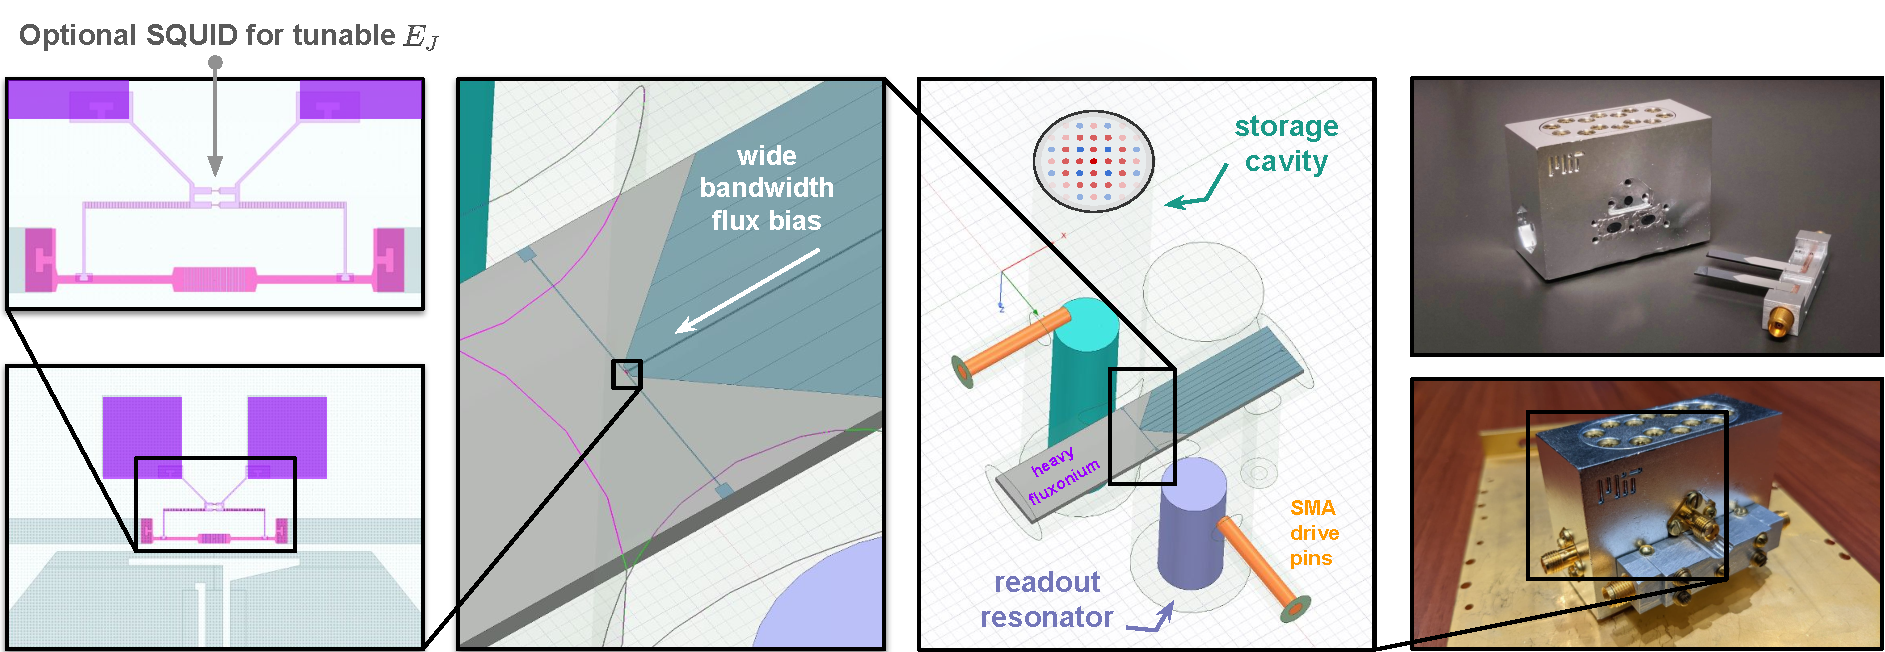
\includegraphics[width=\linewidth]{Figures/4/3DGKP-Schematic.pdf}
    \caption{\todo{Caption}}
    \label{fig:4-3DGKP-schematic}
\end{figure}



\subsection{Cryogenic Setup}

The experiments were performed using a Leiden CF-CS81 dilution refrigerator operated at base temperatures of 8-10 mK. The fridge consists of five temperature stages\footnote{Temperature in the fridge is primarily tracked using three 1 k$\Omega$ platinum (PT-1000) thermometers at the 50K, 3K, and MXC plates, as well as additional capacitive sensors at the MXC. \todo{check!}} as shown in Fig. \ref{fig:4-fridge-wiring}, as well as seven shielding cans that each thermalize to a different temperature stage (not pictured). Specifically, we have two vacuum cans thermalized to room temperature and 1K respectively, and three other cans that provide additional electromagnetic shielding. Finally, to protect against magnetic fields and infrared (IR) radiation, we use two mu-metal shields \todo{check this??} on the coldfinger. A timelapse video of the process to install these cans can be found \href{https://youtu.be/KkvUc9Aw77s?t=829}{here}. 

\begin{figure}[h]
    \centering
    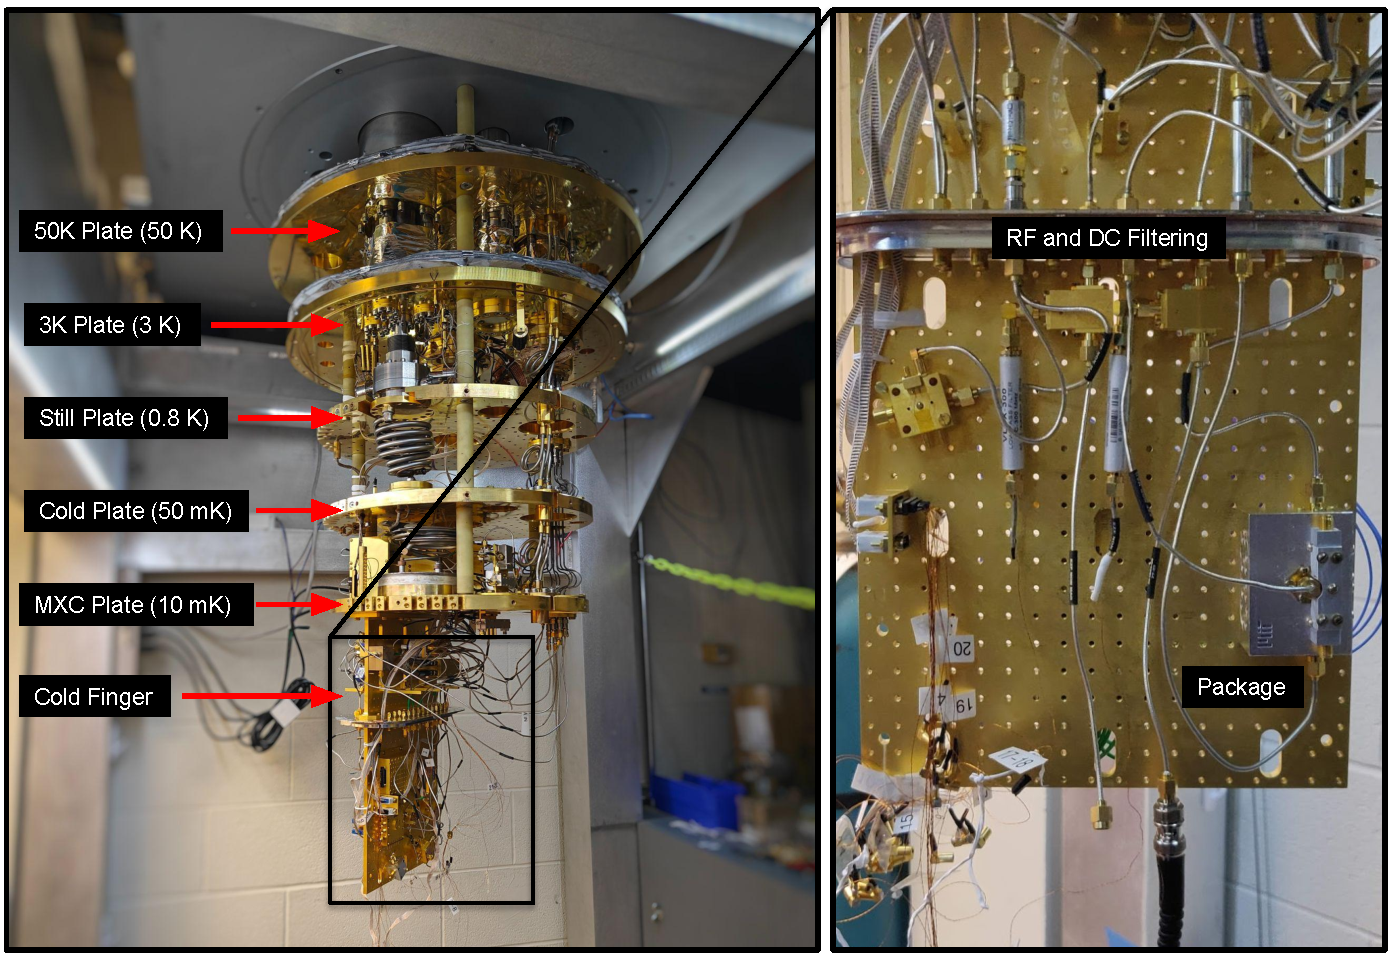
\includegraphics[width=0.9\linewidth]{Figures/4/Fridge-Wiring.pdf}
    \caption{\todo{Caption}}
    \label{fig:4-fridge-wiring}
\end{figure}

The specific experiments presented in this thesis used both DC and radio-frequency (RF) microwave lines to deliver signals to the 3D cavity and fluxonium package. We used three microwave ``drive'' lines for the two fluxonium qubits and the storage resonator, as well as two DC twisted pair connections to provide static flux biasing for the two qubits. The qubit RF and DC signals were first individually filtered and then combined at the mixing chamber through an RF choke. We filtered the DC component using a Mini-Circuits VLFX-300+ low-pass filter, while the RF component was filtered via a K\&L Microwave 12 GHz low-pass filter. This configuration allowed us to probe the higher level transitions of the fluxonium in two-tone spectroscopy through the qubit drive line. 

To attenuate thermal noise coming from the room temperature setup, several attenuators were placed along each of the input microwave lines: a total of 50 dB for the ``drive'' lines and 70 dB for the ``readout'' line. The readout setup had several salient features worth noting: firstly, we used just a single microwave line connected to the two readout cavities via microwave switch; by setting the switch configuration, we selected which of the cavities to measure. Secondly, we used circulators to measure the cavity resonances in reflection. Finally, the reflected output readout signal was pre-amplified using a Josephson travelling wave parametric amplifier (TWPA) at the MXC stage, before being further amplified by a low-noise high-electron-mobility transistor (HEMT) amplifier at 3K, and then a room temperature MITEQ amplifier. The full wiring schematic for this setup is shown below in Fig. \ref{fig:4-microwave-wiring-diagram}. 

\begin{figure}[h]
    \centering
    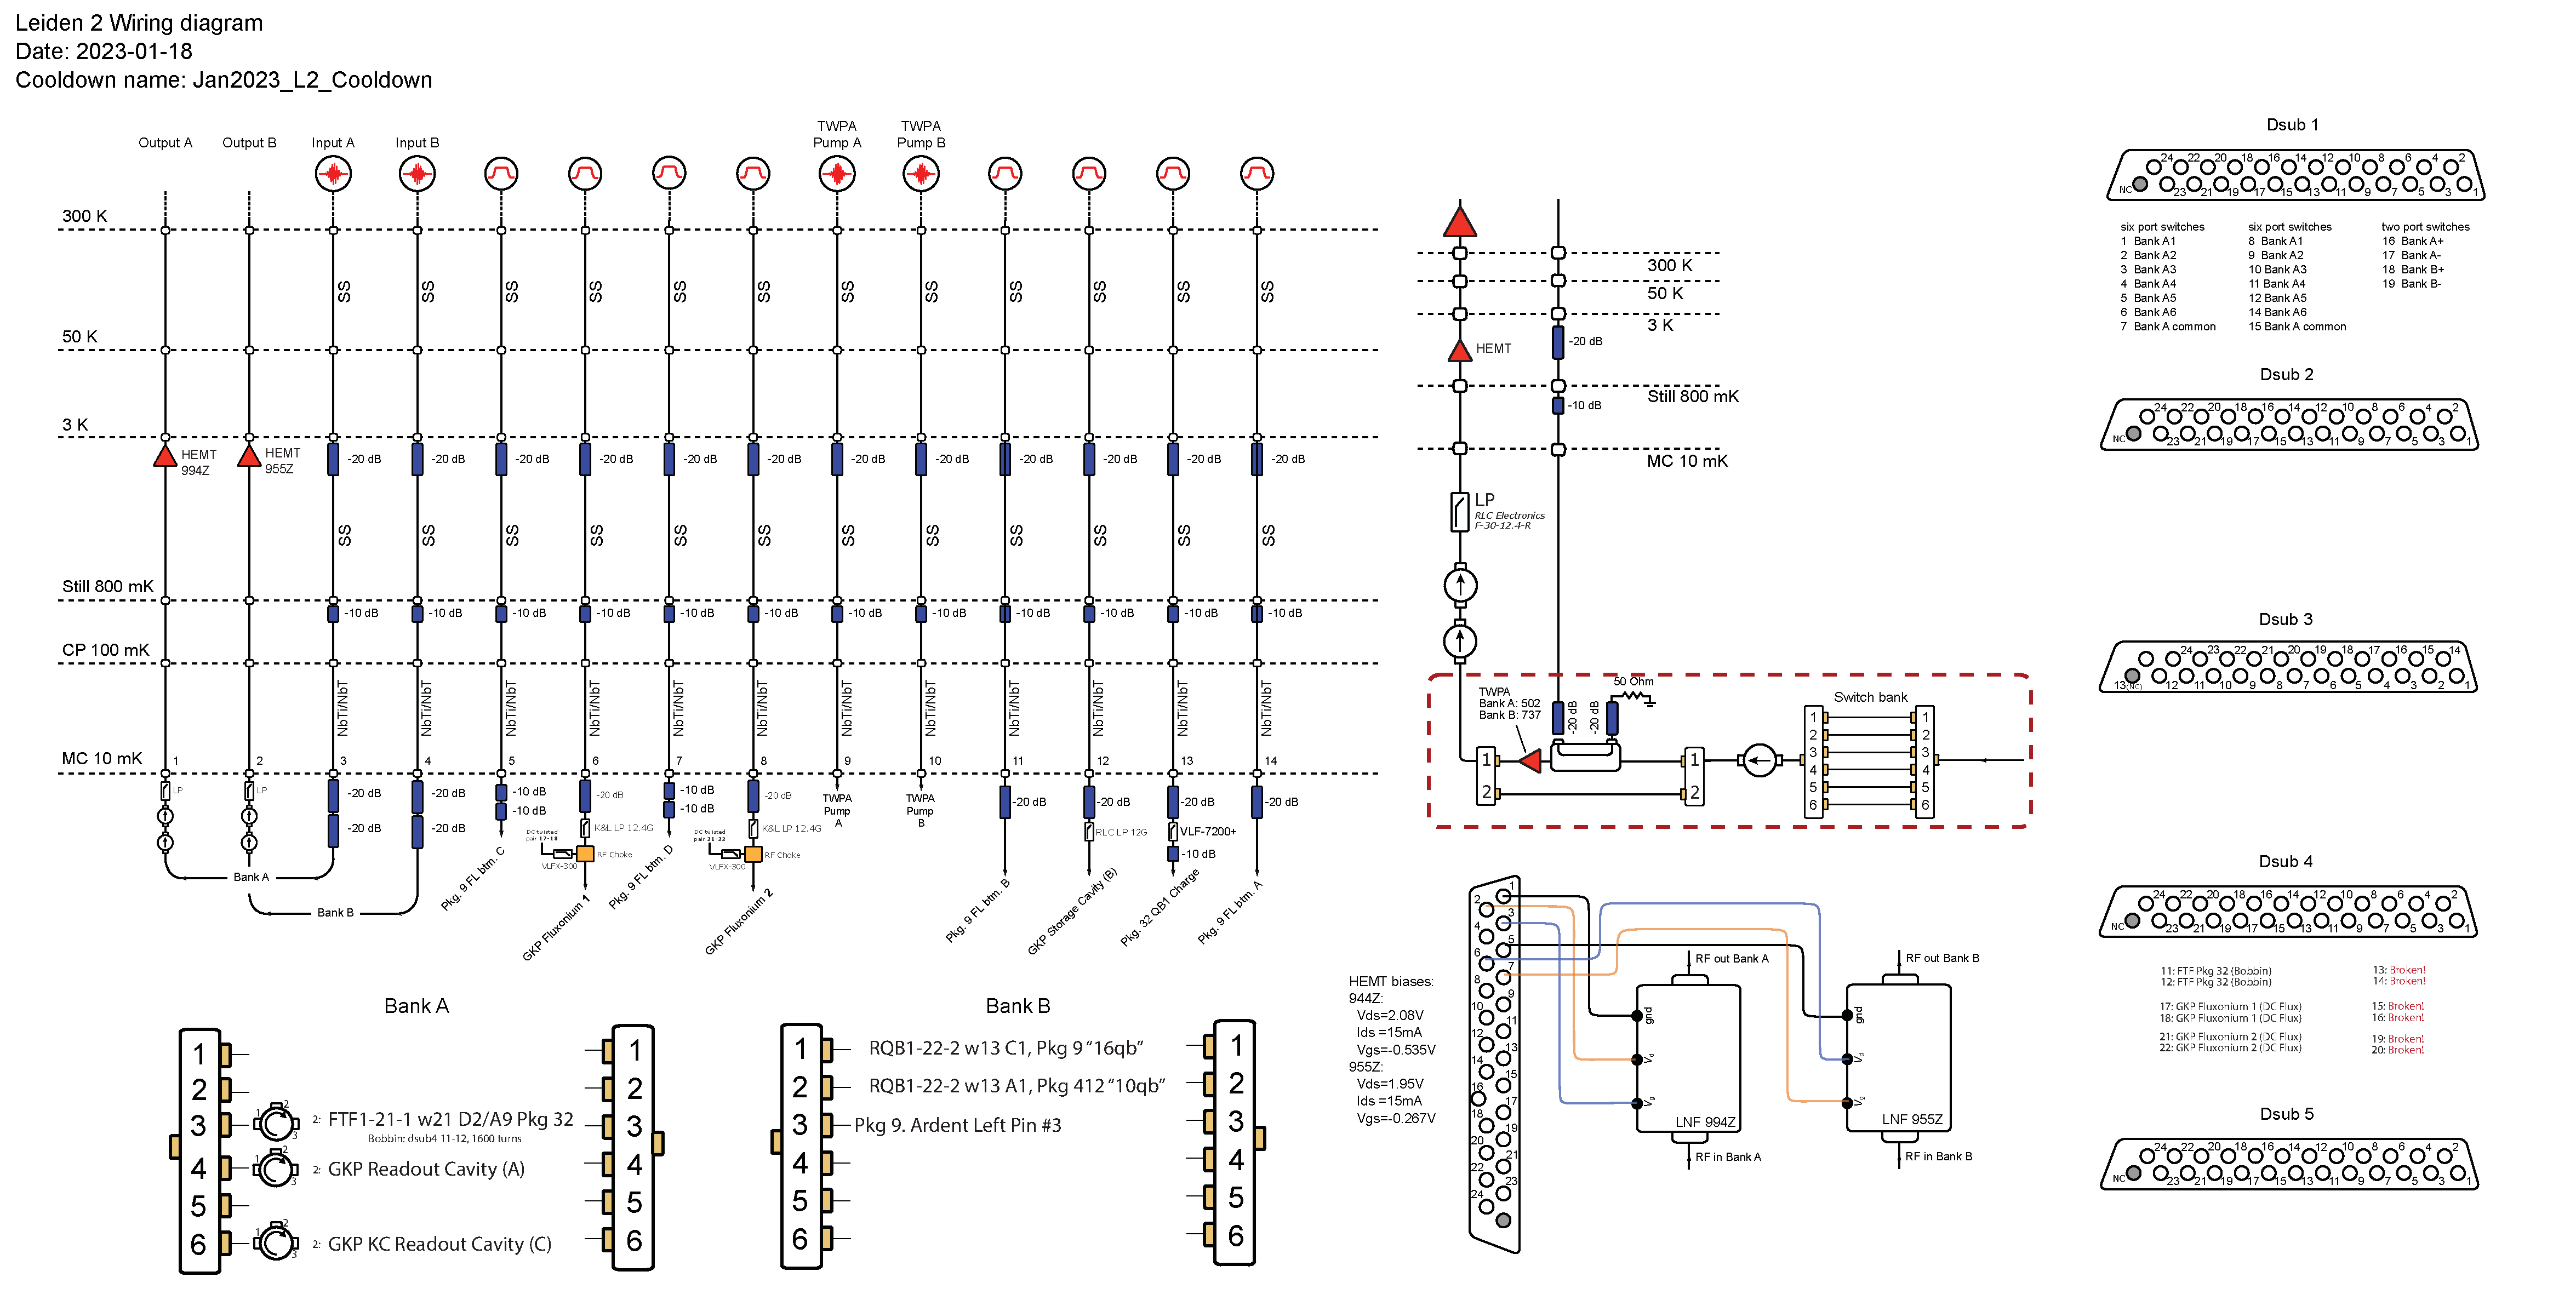
\includegraphics[width=\linewidth]{Figures/4/Microwave-Wiring-Diagram.pdf}
    \caption{\todo{replace image with simplified and corrected version}}
    \label{fig:4-microwave-wiring-diagram}
\end{figure}

At room temperature, pulse waveforms for the various elements were generated using an OPX+ controller from Quantum Machines. For the storage drive, we used an Agilent PSG Signal Generator (E8267D) from Keysight to supply an RF signal which was then combined with the intermediate-frequency (IF) signal from the OPX using the PSG's internal wide-bandwidth IQ mixer. The qubit drive was produced similarly, using a separate Agilent PSG Signal Generator. When performing low-frequency two-tone spectroscopy of the fluxonium $g$--$e$ transition, however, we bypassed the Agilent and instead used baseband signals in the 0-350 MHz range directly from the OPX. Finally, the readout resonator IF signals were generated via the OPX and then passed into a Rohde and Schwarz SGS100A SGMA RF source for upconversion using an internal IQ mixer. The local oscillator (LO) reference signal used for IQ modulation was also passed on to a separate external IQ mixer to demodulate the readout RF output signal coming out of the fridge. The demodulated intermediate-frequency I and Q components were then digitized and processed using the FPGA within the OPX. All microwave signal generators were frequency-locked via a common 10 MHz rubidium clock. 

The DC signals used for static flux biasing were generated via a Yokogawa GS200 Voltage/Current source operated in ``Voltage'' mode; this was then sent into the Qdevil breakout board and then into the fridge via a Fisher cable. Once in the fridge, the signal lines were passed through a resistive DC low-pass filter at the ??K stage \todo{check this!} before terminating in a twisted pair connection. When operating a Yokogawa (or ``Yoko'') in Voltage mode, the DC signal is typically routed through a 1-10 k$\Omega$ resistor to produce an associated current; anecdotally around our lab, this has also been reported to help reduce flux noise from DC lines. However, in the experiments reported below, we mostly chose not to do this and instead used only the bare resistance of the DC line when connected to the fluxonium device, which we measured to be 152.5 $\Omega$ using a multimeter when the fridge was cold. This allowed us to generate a larger current for a given voltage. As we discuss in Sec. \ref{sec:4_Time_Domain}, we later also measured the flux noise amplitude of the qubit when using the ``Current'' mode of the Yoko and found negligible differences in the results. 

\section{Resonator and Two-Tone Spectroscopy}

\textit{In this section, we will present experimental results from our first 3D cavity-fluxonium device with a GKP1 fluxonium chip in our Mark II cavity. We begin with a spectroscopic characterization of the readout resonator and qubit here, followed by time-domain measurements of the qubit in Sec. \ref{sec:4_Time_Domain}, and finally discuss storage resonator measurements in Secs. \ref{sec:4_StorageChi} and \ref{sec:4_StorageCoherenceProblems}. Unless stated otherwise, all data in the upcoming sections was taken using readout cavity A and its associated fluxonium chip. We therefore restrict our focus to the subsystem of the Mark II cavity-fluxonium package comprised of cavity A (readout resonator), fluxonium A (qubit), and cavity B (storage resonator).}

\subsection{Resonator Spectroscopy}
In most circuit QED experiments, the readout resonator forms a crucial gateway through an experimenter probes the system of interest. To this end, the first measurement step we took after cooling down our device was to locate the readout resonator via spectroscopy. As discussed in Sec. \ref{sec:4_3D_Cavity_Resonators}, the readout pin length was chosen here to be overcoupled, with a target coupling rate of $\kappa_c/2\pi \approx 10$ MHz. We were thus able to locate the cavity resonance fairly easily using the VNA and later via pulsed resonator spectroscopy on the OPX with a 10 $\mu$s pulse [see Fig. \ref{fig:4_resonator_spectroscopy}(a)].
\begin{figure}[h!]
    \centering
    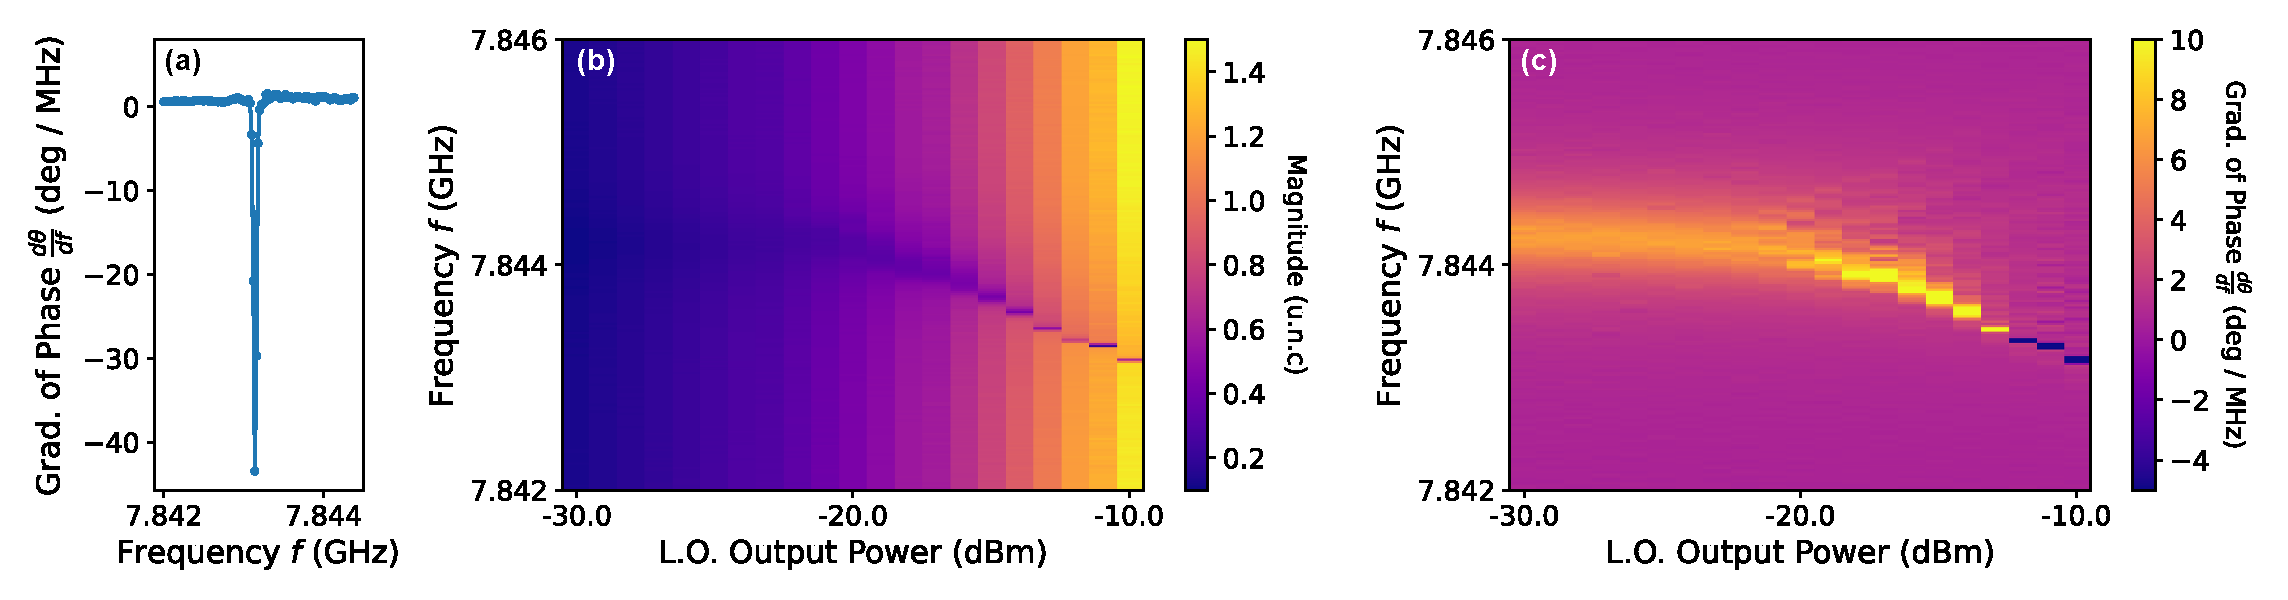
\includegraphics[width=\linewidth]{Figures/4/resonator_spectroscopy.pdf}
    \caption{Caption}
    \label{fig:4_resonator_spectroscopy}
\end{figure}

We next repeated pulsed resonator spectroscopy as a function of the input power of the resonator tone to realize a so-called ``punchout'' measurement [Fig. \ref{fig:4_resonator_spectroscopy}(b-c)]. In the data, we observe the resonator ``punching'' out, i.e. its frequency shifting downwards towards its bare value as we increase the drive power and decouple from the nonlinear degrees of freedom in the system (e.g. the qubit or antenna mode here). Punchout is typically used as a way to check whether a qubit is alive, since the nonlinearity of the qubit directly results in a nonlinear response in the resonator. For a practical explanation of this, I refer interested readers to Ref. \cite{naghiloo2019introduction}, which also gives a step-by-step experimentalist's introduction to qubit measurements in circuit QED. 

Due to its coupling to the fluxonium qubit, we also expect the resonator to inherit some flux dependence in addition to nonlinearity. Therefore, after verifying that the resonator frequency changes with power, we next performed resonator spectroscopy vs. the applied external flux bias on the qubit [see Fig. \ref{fig:4_resonator_spectroscopy_vs_flux}]. We set the bias using the room temperature Yokogawa source to set voltage (which induced a current through the DC line, and in turn generated an applied flux through the fluxonium loop). After setting each bias voltage, we waited for 0.1s for the flux to settle and then performed resonator spectroscopy.  

\begin{figure}[h]
    \centering
    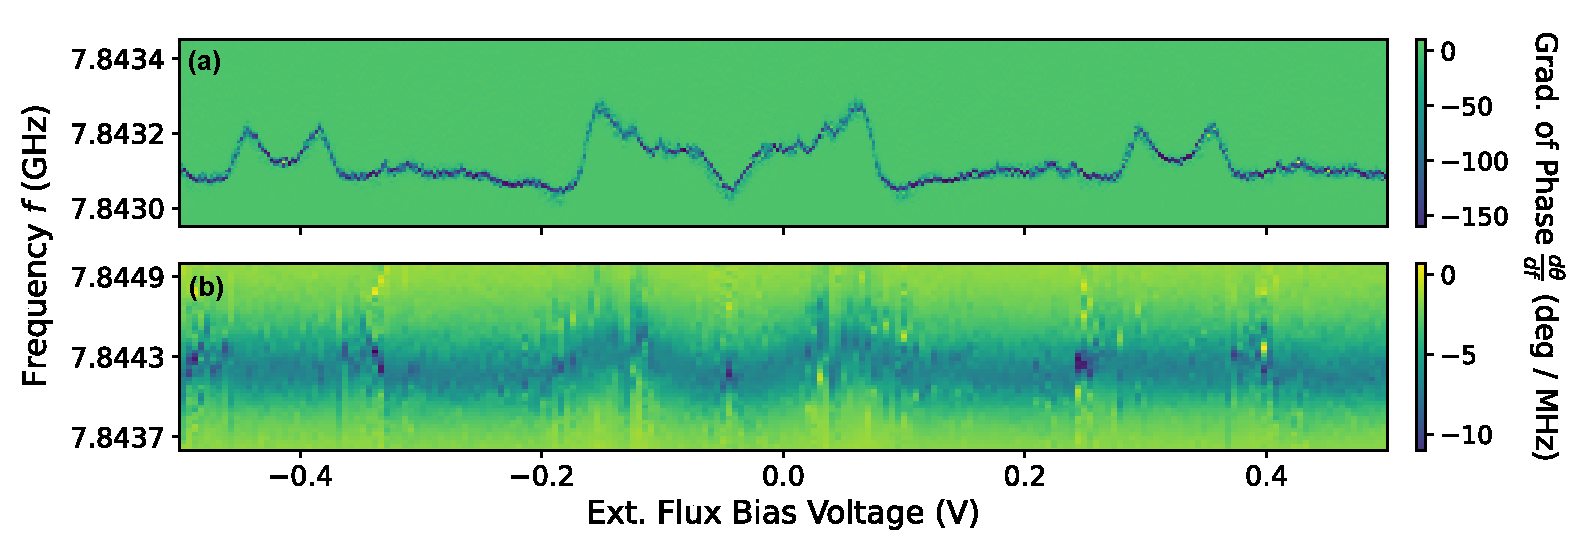
\includegraphics[width=\linewidth]{Figures/4/resonator_spectroscopy_vs_flux.pdf}
    \caption{Caption}
\label{fig:4_resonator_spectroscopy_vs_flux}
\end{figure}

We see that the the resonator frequency indeed varies periodically with the bias voltage. From the periodicity of the spectrum, we found (and later corroborated via qubit two-tone spectroscopy measurements) that a flux quantum in this device corresponds to 4.872 mA, realized in this configuration via a voltage of about 0.743 V applied over the line resistance of 152.5 $\Omega$. The resonator spectrum is expected to be symmetric about both zero external flux ($\Phi_{\rm ext} = 0$) and ``half-flux'' ($\Phi_{\rm ext} = \Phi_0/2$), and we can observe two symmetry points above --- one at $V_b \approx -0.045$ V, and other at both $V_b \approx 0.326$ V and $V_b \approx -0.414$ V. From the averaged data in Fig. \ref{fig:4_resonator_spectroscopy_vs_flux} alone, it is rather difficult to identify which of these symmetry points corresponds to ``half-flux''. However, we can make this identification by instead working with single-shot data, i.e. not directly averaging across shots on the OPX during readout. At $\Phi_{\rm ext} = 0$, the fluxonium has a single ground state $\ket{g}$ that the qubit relaxes to in thermal equilibrium. Thus the dispersive readout will result in a \textit{single} ``I-Q blob'' in the demodulated signal. However, at $\Phi_{\rm ext} = \Phi_0/2$, both the ground and excited states will be thermally occupied in equilibrium due to the low-frequency nature of the qubit \cite{manenti2023quantum}, and thus we expect to see two ``blobs'' in the I-Q plane corresponding to the qubit initial state being in either $\ket{g}$ or $\ket{e}$. When we set the Yoko voltage to $V_b = -0.04465$ V, the single-shot data [cf. Fig \ref{fig:4_single_shots}] reveals two IQ ``blobs'' in the histogram, confirming that this bias point is, in fact, the half-flux sweet spot. (By association the other symmetry points correspond to \textit{integer} flux quanta). Therefore, using our calibration of the flux axis, we can map between the bias voltage and the applied external flux $\Phi_{\rm ext}$ in subsequent measurements. 

\begin{figure}[h]
    \centering
    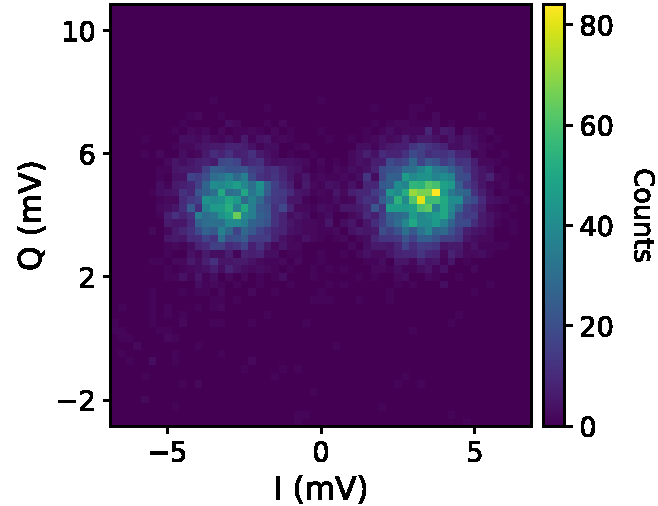
\includegraphics[width=0.6\linewidth]{Figures/4/single_shots.pdf}
    \caption{Histogram of 10,000 digitized single-shot readout measurements, plotted in the I-Q plane. The two ``blobs'' correspond to the two qubit states $\ket{g}$ and $\ket{e}$ that will both be populated in equilibrium when the fluxonium is parked near the half-flux sweet spot.}
\label{fig:4_single_shots}
\end{figure}


\newpage
\subsection{Two-Tone Spectroscopy}
After characterizing the resonator, our next step was \textit{two-tone spectroscopy} (also called qubit spectroscopy). Here, the two ``tones'' in question are (i) a qubit drive tone to probe transitions of the fluxonium, followed by (ii) a resonant readout tone. Practically, we can understand a two-tone spectroscopy experiment as follows by considering the dispersive Hamiltonian \cite{zhu2013cQEDfluxonium}:
\begin{equation}
    \hat{H} = \sum_k \tilde{E}_k \op{k}{k} + \bigg(\omega_r^0 + \sum_k \chi_k \op{k}{k}\bigg) \hat{a}^\dagger\hat{a}
\end{equation}
We have Lamb-shifted qubit energies $\tilde{E}_k$ and eigenstates $\ket{k}$, as well as a resonator whose frequency $\tilde{\omega}_r$ (in parentheses) depends on the qubit state. For the sake of illustration, let's briefly work near zero flux so that only the ground state $\ket{g}$ is initially populated in thermal equilibrium. The basic idea of the experiment is to play a weak continuous spectroscopy (or ``\textit{saturation}'') tone on the qubit. As we sweep the frequency, we'll eventually come into resonance with a qubit transition, e.g. $f_{gl}$ between $\ket{g}$ and some other state $\ket{l}$. When this happens, the resonant tone has the effect of driving Rabi oscillations between the states $\ket{g} \leftrightarrow \ket{l}$; furthermore, over many multiples of the coherence time, the qubit state will also change due to $T_1$ relaxation and/or heating processes. As a result, the qubit will be left in a non-equilibrium (i.e. driven, dissipative) steady state $\hat{\rho}$ with occupation probabilities $p_k$. Due to the dispersive interaction, this mixed state in turn leads to a final average resonator frequency 
\begin{equation}
    \ev{\tilde{\omega}_r}_{\rm final} = \omega_r^0 + \Tr\bigg(\hat{\rho} \sum_k \chi_k \op{k}{k}\bigg) = \omega_r^0 + \sum_k p_k \chi_k
\end{equation}
that is different from the initial one, i.e. $\ev{\tilde{\omega}_r}_{\rm init} = \omega_r^0 + \chi_g$. Using a resonator measurement, we can then detect this change in the resonance frequency (e.g. by measuring the change in signal phase when ``reading out'' at a fixed frequency $\ev{\tilde{\omega}_r}_{\rm init}$), and so map out the qubit transitions. If we now do this as a function of flux, the initial qubit state may also need to be described by a mixed state, e.g. a thermal mixture of $\ket{g}$ and $\ket{e}$ near half-flux; nevertheless, as long as the initial and final mixed states lead to different average resonator frequencies, we will be able to identify that a transition has occurred. 

In experiment, we performed wideband two-tone spectroscopy to map out the higher energy transitions of the fluxonium versus external flux. The full spectrum is shown below in Fig. \ref{fig:4_two_tone_vs_flux_full}, and we already see a rich set of features in the data. The qubit transitions have a clear dependence on flux, and are notably symmetric about the two sweet spots at $\Phi_{\rm ext} = 0$ and $\Phi_{\rm ext} = \Phi_0/2$. In panel (b), we overlay a theoretical prediction obtained from numerical diagonalization of the fluxonium Hamiltonian with free parameters $E_C$, $E_J$, and $E_L$. We extract
\begin{equation}
    E_C/h \approx 1.678 \,\, \text{GHz}, \quad  E_J/h \approx 8.987 \,\, \text{GHz}, \quad  E_L/h \approx 0.342 \,\, \text{GHz} 
    \label{eq:4_qubit_parameters_fit}
\end{equation}
as the qubit parameters for this device by fitting to the data. This is within the range that we designed for, and results in a qubit frequency of approximately 94.1 MHz at half-flux. 

At this resolution, there are also certain features that appear to be constant with flux. We can identify these are the various linear modes in the system, e.g. the storage resonator at 8.86 GHz, and the two on-chip antenna modes at 8.60 GHz and 8.46 GHz. Since each of these modes has a dispersive shift to the readout resonator (also shown), we are able to see them in this two-tone measurement just as we do the other qubit transitions\footnote{We can also see some other faint qubit-like transitions near half-flux. We will comment on these later, as they are actually quite interesting: we'll see that they are two-photon ``parasitic'' qubit-resonator transitions.}. Note that each of these linear modes (including the readout) has \textit{some} flux dispersion if we zoom in close enough. This is important for readout calibration, as typically the readout frequency must be calibrated at each new flux operating point. In the data shown here, we did not do this, and instead used a constant frequency tone at 7.8442 GHz, which was approximately resonant across the entire flux range (cf. low-power data in Fig. \ref{fig:4_resonator_spectroscopy_vs_flux}). While this worked reasonably well, we nonetheless see variations in readout constant that could be improved by first redoing resonator spectroscopy at each flux point prior to two-tone, or by creating a lookup table ahead of time. 

From the wideband spectrum (also cf. Fig. \ref{fig:4_two_tone_vs_flux_zoom} below), we can clearly see that the storage resonator frequency lies between the two sets of fluxonium plasmon transitions. This is precisely what we had hoped to engineer in our system: as a reminder, we will refer to this important condition as bosonic mode threading. 

\begin{figure}[hp]
    \centering
    \includegraphics[width=0.95\linewidth]{Figures/4/two_tone_vs_flux_full.pdf}
    \caption{Caption}
\label{fig:4_two_tone_vs_flux_full}
\end{figure}
\clearpage

\begin{figure}[hp]
    \centering
    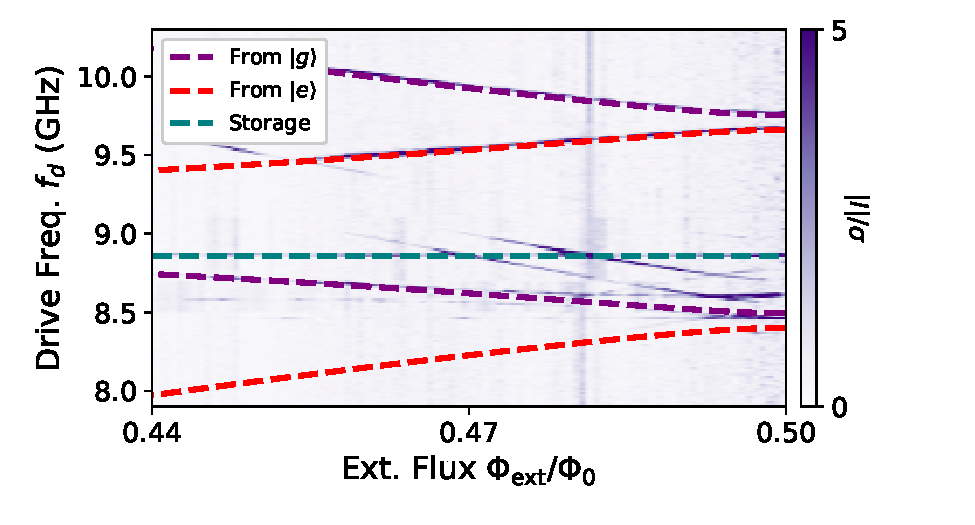
\includegraphics[width=0.8\linewidth]{Figures/4/two_tone_vs_flux_zoom.pdf}
    \caption{Zoomed-in two-tone spectroscopy showing bosonic mode threading, with the storage resonator frequency in between the two sets of fluxonium plasmon transitions. Dashed lines from $\ket{g}$ and from $\ket{e}$ show theoretical predictions from numerical diagonalization of the qubit, as before. The storage flux dispersion cannot seen at this resolution.}
\label{fig:4_two_tone_vs_flux_zoom}
\end{figure}

Our next experimental step was low-frequency qubit spectroscopy near half-flux using a direct baseband drive to map out the qubit  $\ket{g}\to\ket{e}$ transition: we show the data below in Fig. \ref{fig:4_qubit_spectroscopy}. Unlike prior measurements, here we used a dual readout post-selection scheme \cite{ding2023FTF} to improve contrast and assign an occupation probability to the qubit. This was crucial to obtain our results, and we will discuss it further in the upcoming section.

\begin{figure}[!b]
    \centering
    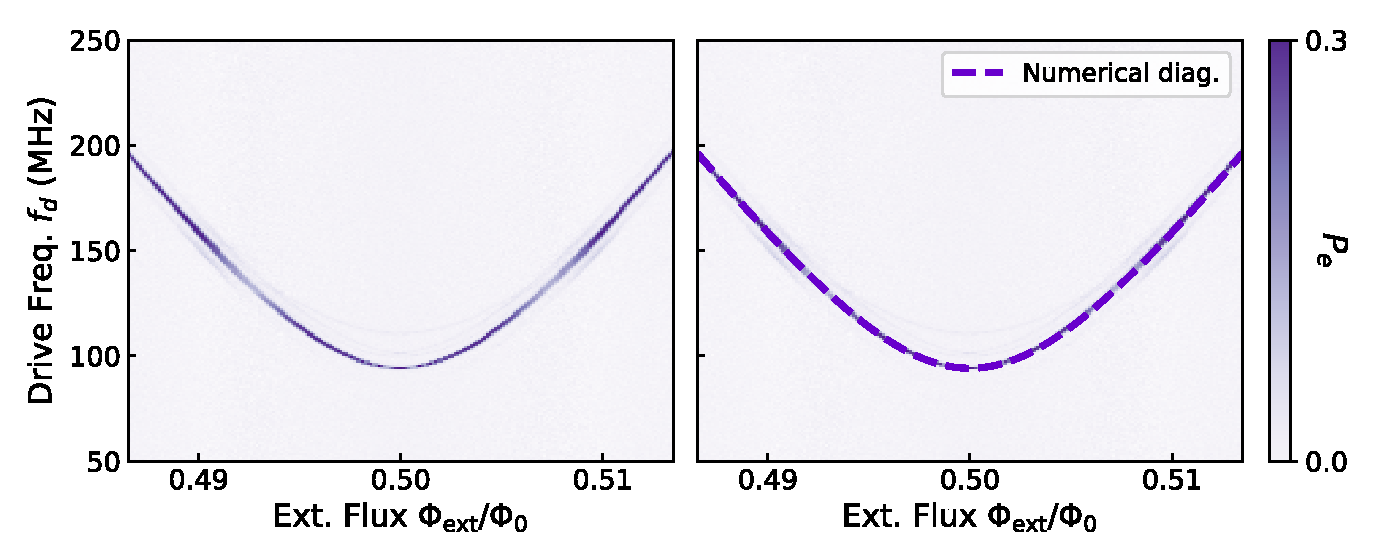
\includegraphics[width=0.9\linewidth]{Figures/4/qubit_spectroscopy.pdf}
    \caption{Post-selected baseband two-tone spectroscopy showing the fluxonium $\ket{g}\to\ket{e}$ transition with and without the theoretical fit from numerical diagonalization using the same parameters as before [Eq. \eqref{eq:4_qubit_parameters_fit}]. At half-flux, the qubit frequency is 94.1 MHz.}
\label{fig:4_qubit_spectroscopy}
\end{figure}

\section{Time-Domain Measurements of the Qubit \label{sec:4_Time_Domain}}

\subsection{Post-Selection via Single-Shot Readout}

Near half-flux, the energy of the fluxonium qubit transition $\h\omega_q$ can be much smaller than the ambient temperature $k_BT$ of a typical dilution refrigerator. As a result, the fluxonium in equilibrium will be in a thermal mixture of $\ket{g}$ and $\ket{e}$; we saw this in Fig. \ref{fig:4_single_shots} already. For our specific parameters of $f_q = 94.1$ MHz and $T = 9$ mK, the excited state population is given by a Boltzman distribution: $p_e \simeq 1 / (e^{\h\omega_q/k_B T} + 1) \approx 60\%$. For the higher-level (i.e. wideband) two-tone spectroscopy above, this initial thermal distribution was not a problem --- on the contrary, starting from a mixed state is even beneficial, allowing us to see transitions out of both $\ket{g}$ and $\ket{e}$. However, for baseband qubit spectroscopy probing the $\ket{g}\leftrightarrow\ket{e}$ transition, and critically also for time-domain experiments, this ceases to be true. For these measurements, we instead want to be able to discriminate between the two states. In our experiments, the approach we chose to do this was single-shot readout and post-selection. We specifically followed the dual readout scheme discussed in Refs. \cite{ding2023FTF, ding2023thesis} (cf. Fig. \ref{fig:4_postselection} below)\footnote{At this point, I'd also sincerely like to thank Leon Ding for his early guidance with fluxonium experiments!}. Here, the first readout pulse initializes the fluxonium state to either $\ket{g}$ or $\ket{e}$ via projective measurement. We then start the rest of the experimental sequence (e.g. qubit pulses, delays, storage pulses) from a known initial state, and finally conclude with a second readout pulse to record the qubit state. All the time-domain measurements that follow used this post-selected sequence. 

\begin{figure}[b!]
    \centering
    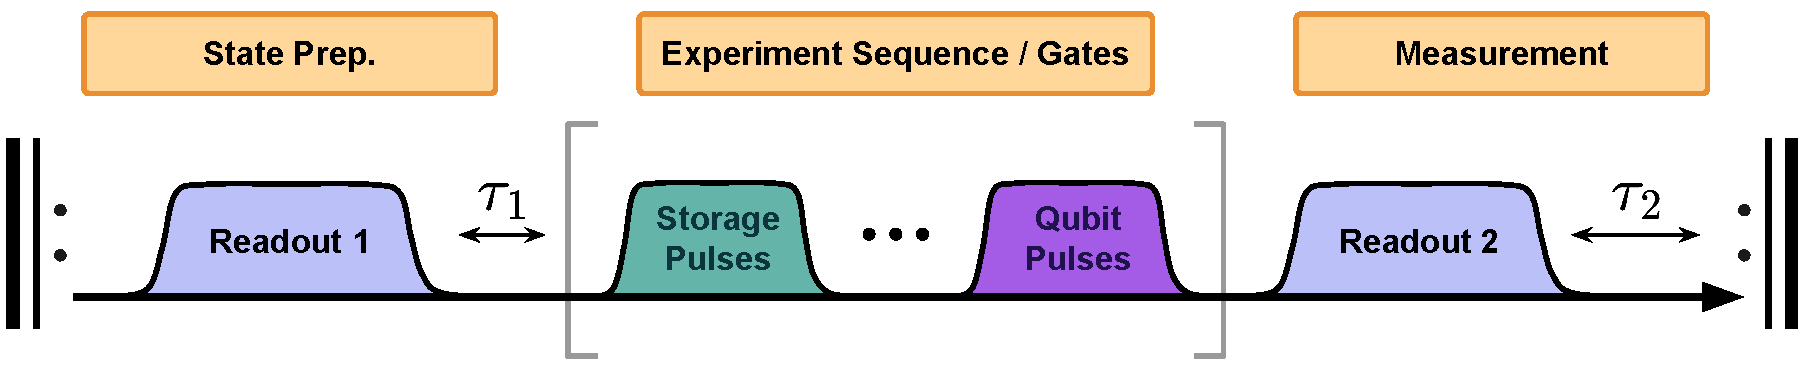
\includegraphics[width=0.9\linewidth]{Figures/4/postselection.pdf}
    \caption{Dual readout post-selection. Here, the first readout prepares the qubit in $\ket{g}$ or $\ket{e}$ and the second readout records the final qubit state after performing the experiment sequence. We introduce a short ring-down time $\tau_1$ to allow readout photons to decay after the first readout, and a longer delay $\tau_2$ to let the qubit relax to equilibrium between shots.}
    \label{fig:4_postselection}
\end{figure}
\clearpage

\subsection{Rabi Oscillations and Pi Pulse Calibration}

After having identified the qubit frequency in two-tone spectroscopy, we next turned to time-domain experiments involving coherent manipulation of the qubit state. The first of these was, of course, to demonstrate Rabi oscillations between the $\ket{g}$ and $\ket{e}$ states using a resonant drive. In heavy fluxonium, the $T_1$ protection that arises due to the small charge matrix element also has the effect of making it generically more difficult to drive the associated transitions. As a result, several previous experiments with fluxonium or other low-frequency flux qubits have had to use either non-adiabatic Landau-Zener flux control \cite{oliver2005mach, campbell2020universal, zhang2021universal}, or virtual (Raman) transitions mediated by a higher energy state \cite{earnest2018realization}. Thankfully, we were able to use more conventional microwave-based control via a resonant drive, since our device was not quite so heavy. 

In Fig. \ref{fig:4_rabi}, we show a typical \textbf{power Rabi} measurement, taken with the qubit parked at half-flux. For this data, we specifically used a fixed length ($\tau = 200$ ns) Gaussian pulse whose amplitude we swept to generate Rabi oscillations: this is shown below on the left for a resonant drive. Meanwhile, on the right, we have a characteristic ``chevron'' plot. By finding the point of minimum contrast in the 2D sweep of Rabi frequency and amplitude, we can tune up $\pi$- and $(\pi/2)$-pulses on the qubit. 

\begin{figure}[h]
    \centering
    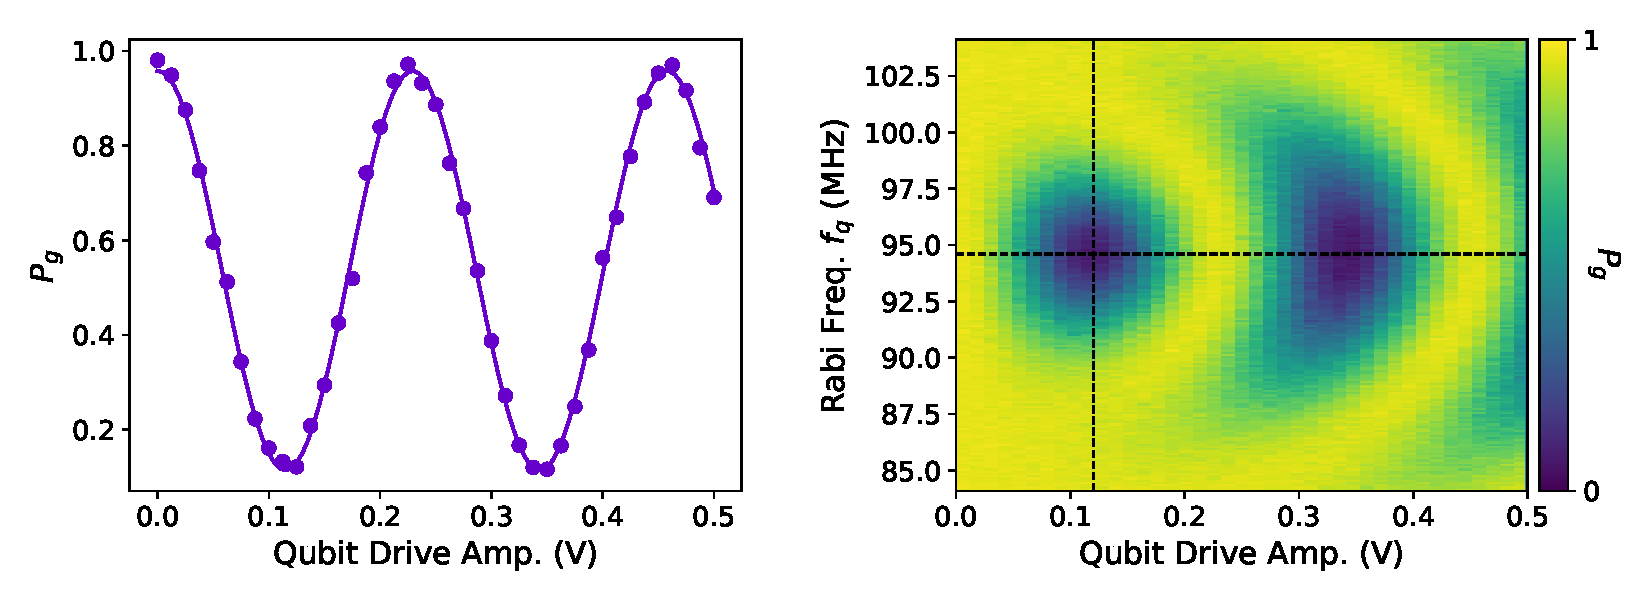
\includegraphics[width=0.95\linewidth]{Figures/4/rabi.pdf}
    \caption{Caption}
    \label{fig:4_rabi}
\end{figure}

In subsequent measurements, we typically tuned up two kinds of $\pi$-pulses: the first was a shorter $\tau = 48$ ns pulse, which we used in most of the time-resolved qubit experiments. The second was a ``selective'' qubit pulse, of length $\tau = 2.4$ $\mu$s, chosen so that the associated spectral bandwidth of the pulse $1/\tau$ was smaller (at least at half-flux) than the dispersive shift $\chi$ between the qubit and storage mode (cf. Sec \ref{sec:4_StorageChi} where we discuss this further). We also later switched from Gaussian to cosine pulses; the latter were easier to work with due to their well-defined end points (zero amplitude at the start and end of the pulse). 

\subsection{Measuring the Fluxonium \texorpdfstring{$T_1$}{T1}}

Our next set of experiments involved measuring the $T_1$ relaxation time of the fluxonium. The post-selection sequence we used to realize the measurement consists of two readouts separated by a variable length delay. The first readout initializes the qubit in either $\ket{g}$ or $\ket{e}$, while the second is used to track a change of state. The result is a characteristic $T_1$ relaxation curve showing an exponential decay of the qubit populations with time. We show an example of such a curve in Fig. \ref{fig:4_qubit_T1_vs_flux_single}(a), from which we extract a decay constant $T_1 = 220 \pm 10$ $\mu$s. Panel (b) shows the results of the same experiment now repeated across various external flux biases: we see that the flux-dependence of the qubit $T_1$ is very sharply peaked and symmetric about half-flux, with a maximum value of $T_1 \approx 265$ $\mu$s.

\begin{figure}[h]
    \centering
    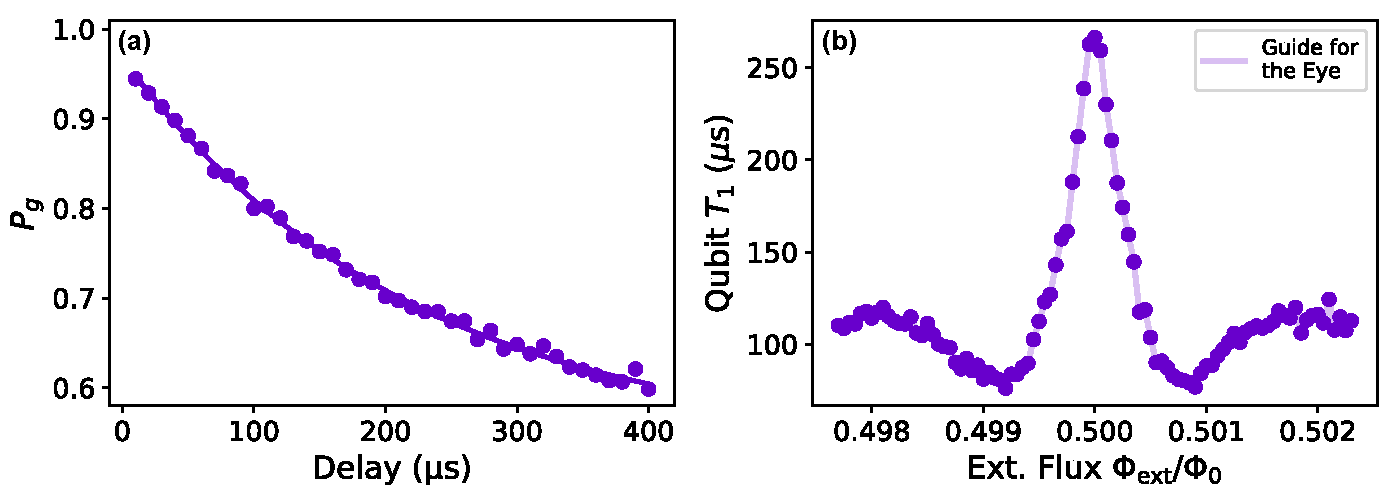
\includegraphics[width=0.95\linewidth]{Figures/4/qubit_T1_vs_flux_single.pdf}
    \caption{Caption}
    \label{fig:4_qubit_T1_vs_flux_single}
\end{figure}

The sharply peaked flux-dependence in Panel \ref{fig:4_qubit_T1_vs_flux_single}(b) was one of the first experimental mysteries that we encountered with this device. For the parameters of our fluxonium, and assuming a capacitive (i.e. dielectric) loss model, we naively expected $T_1$ to improve away from half-flux. There are other loss models that would predict $T_1$ degrading away from half-flux (e.g. quasiparticle tunneling); however, we were unable to reproduce the sharp initial drop-off in any numerical simulations at the time of the experiment. [As we discuss below, however, we have since come up with a model that we believe may explain these observations]. 

If we go out even further in flux, we see an even richer structure to the flux-dependence of the fluxonium $T_1$ [see Fig. \ref{fig:4_qubit_T1_vs_flux_spec}]. Away from half-flux, we see a clear drop in $T_1$, followed by an apparent revival around $\Phi_{\rm ext} \approx 0.485\Phi_0$. However, as we move leftwards, we again see further drop-offs in the $T_1$. Although these observations puzzled us for some time, we eventually came to the hypothesis that the drop-offs in $T_1$ may be a form of Purcell decay.

\begin{figure}[h]
    \centering
    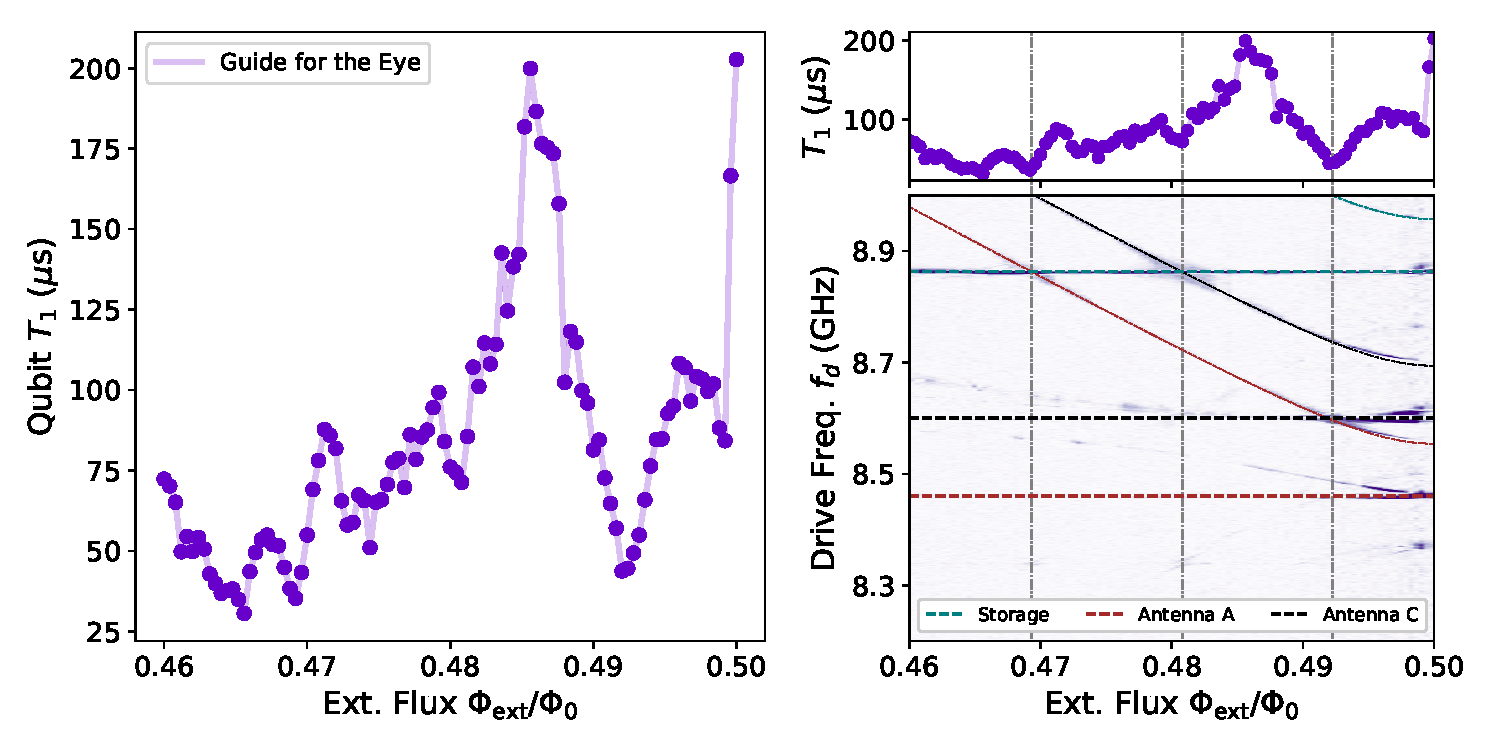
\includegraphics[width=0.95\linewidth]{Figures/4/qubit_T1_vs_flux_spec.pdf}
    \caption{Caption}
    \label{fig:4_qubit_T1_vs_flux_spec}
\end{figure}

In the right panel of Fig. \ref{fig:4_qubit_T1_vs_flux_spec}, we reproduce the $T_1$ data from the left panel, but also now align it with two-tone spectroscopy data taken earlier. At this resolution, the storage and the two antenna modes are straight lines. On top of these we see certain flux-dependent transitions: it turns out that these are ``two-photon'' transitions! (We showed these in Fig. \ref{fig:4_two_tone_vs_flux_full} as well). Specifically, they correspond to the frequencies of the linear modes \textit{plus} the qubit $\ket{g}\to\ket{e}$ frequency, i.e. they are activated in two-tone spectroscopy when $\omega_d \approx \omega_{\rm lin} + \omega_{ge}$ where $\omega_{\rm lin}$ can be the frequency of the storage or either antenna. Intuitively, we can understand the drop-offs in qubit $T_1$ occurring when this transition is tuned into resonance with one of the other linear modes. For example, near $\Phi_{\rm ext} \approx 0.48\Phi_0$, we have the resonance $\omega_{\rm ant.\,C} + \omega_{ge} \approx \omega_{s}$ 



\subsection{Coherence Measurements: Ramsey and Echo}






\subsection{Flux Noise Amplitude Characterization}


\section{Storage Resonator Measurements \label{sec:4_StorageChi}}

\subsection{Storage Spectroscopy}

\subsection{Engineering a Tunable Dispersive Shift}

\section{Storage Coherence: Problems and Pitfalls \label{sec:4_StorageCoherenceProblems}}

